\texttt{Alfa-Beta}
\begin{figure}[h]
    \centering
    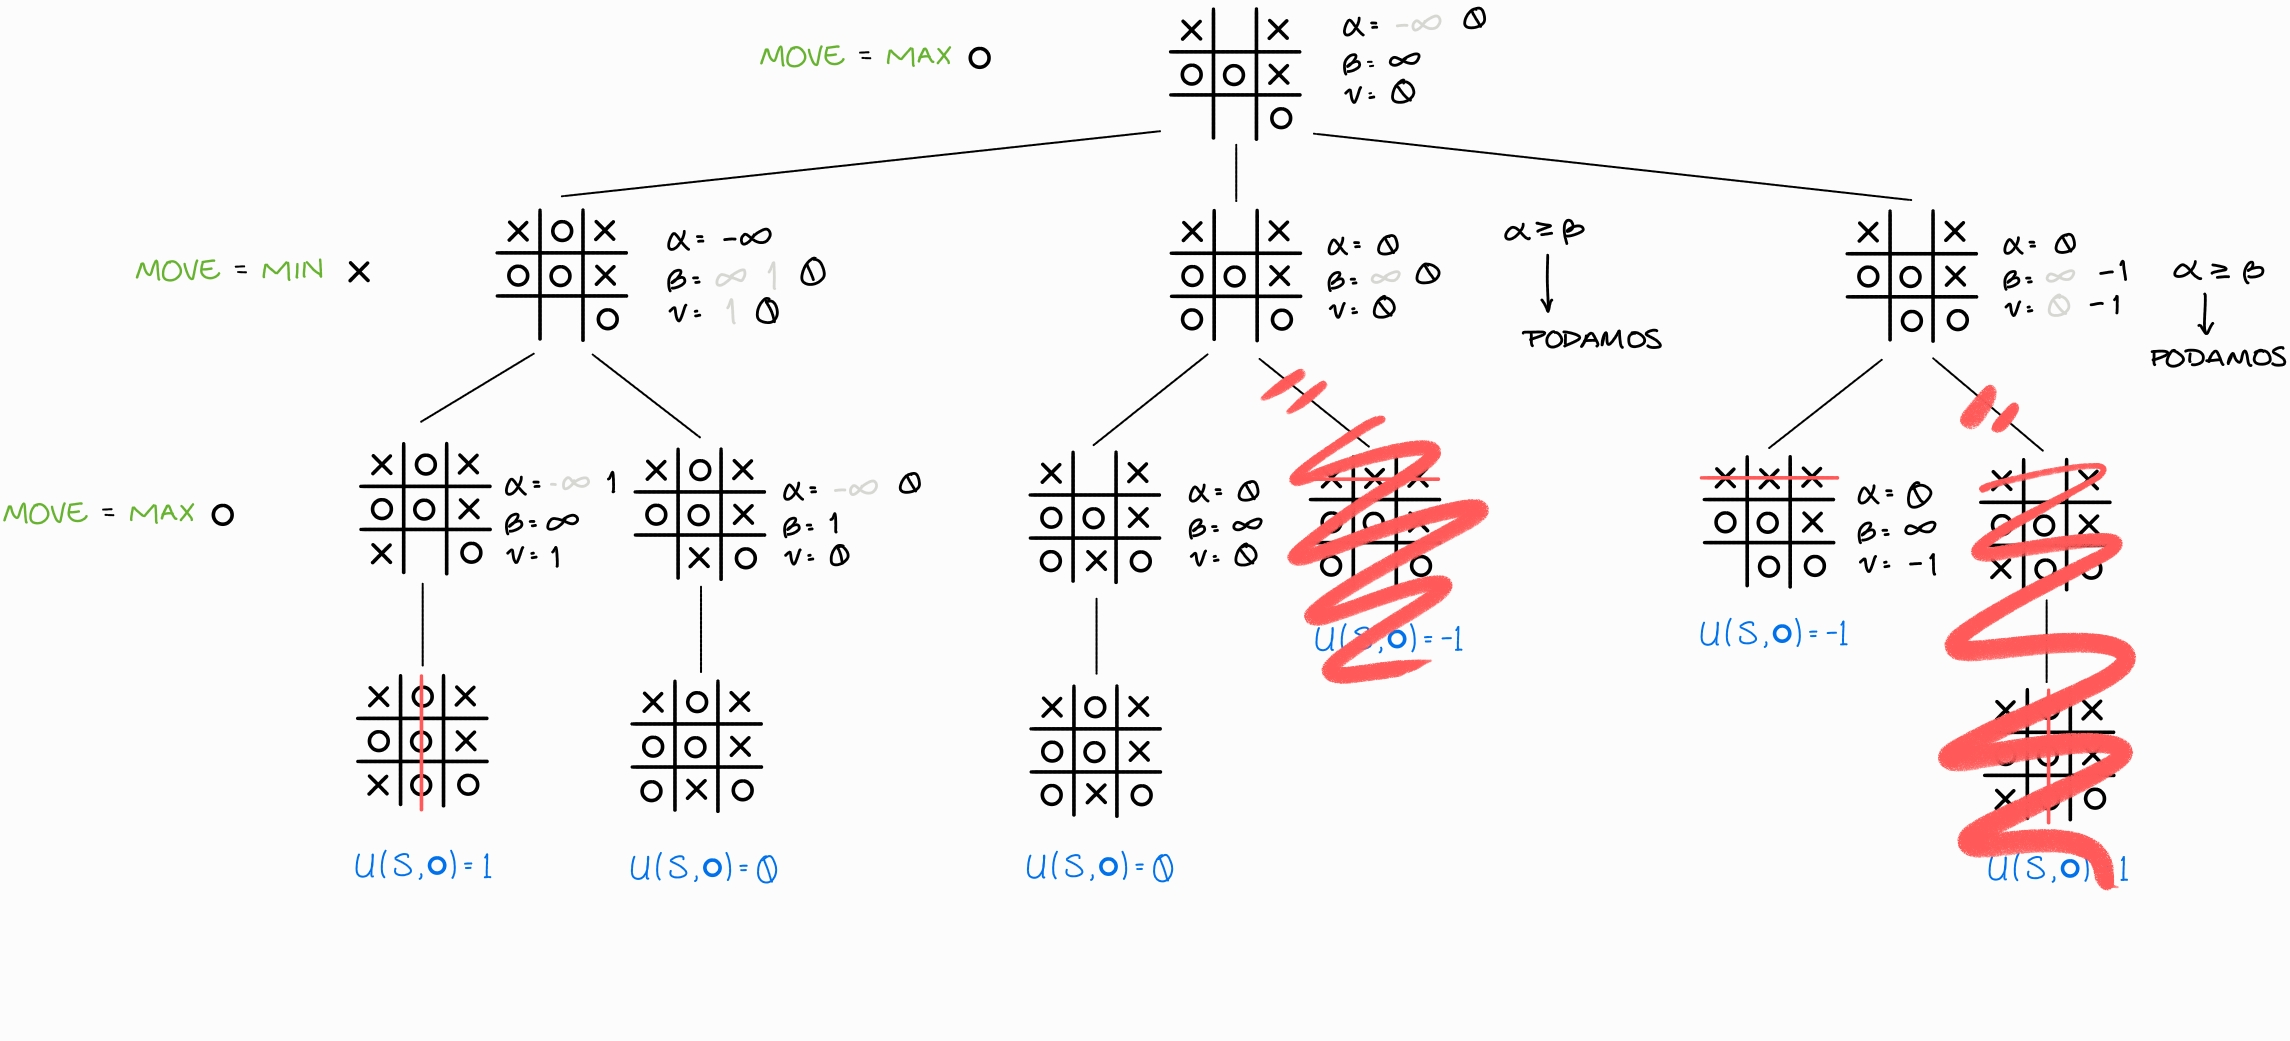
\includegraphics[width=1\textwidth]{f2_e11.jpg}
\end{figure}

En la raíz (nodo MAX) iniciamos con

\[
\alpha=-\infty, \qquad \beta=\infty.
\]

Exploramos los hijos de izquierda a derecha.

\begin{enumerate}

\item \textit{Primer hijo de la raíz (nodo MIN).}

Este nodo corresponde al turno de $X$. Sus dos hijos son nodos MAX.

\begin{itemize}
\item El primer nodo MAX nos lleva a un estado terminal con utilidad
\[
U(S,O)=1.
\]

\item El segundo nodo MAX nos lleva a un estado terminal con utilidad
\[
U(S,O)=0.
\]
\end{itemize}

Como este nodo es MIN, toma el mínimo de sus hijos:

\[
v=\min(1,0)=0.
\]

Este valor se propaga a la raíz. Como la raíz es MAX, actualizamos

\[
\alpha=\max(-\infty,0)=0.
\]

\item \textit{Segundo hijo de la raíz (nodo MIN).}

Este nodo hereda

\[
\alpha=0, \qquad \beta=\infty.
\]

Evaluamos su primer sucesor (nodo MAX), que lleva a un estado terminal con

\[
U(S,O)=0.
\]

Entonces

\[
\beta=\min(\infty,0)=0.
\]

En este momento se cumple

\[
\alpha \ge \beta \qquad (0 \ge 0),
\]

por lo que se \texttt{poda} y el resto de los hijos de este nodo
no se exploran.

\item \textit{Tercer hijo de la raíz (nodo MIN).}

Este nodo también recibe

\[
\alpha=0, \qquad \beta=\infty.
\]

Evaluamos su primer sucesor (nodo MAX), que lleva a un estado terminal con

\[
U(S,O)=-1.
\]

Entonces

\[
\beta=\min(\infty,-1)=-1.
\]

Se cumple nuevamente

\[
\alpha \ge \beta \qquad (0 \ge -1),
\]

por lo que se \texttt{podan} los demás sucesores de este nodo.

\end{enumerate}

El algoritmo $\alpha$-$\beta$ evita evaluar varias ramas del árbol.
